\rhschapter{Testing}

\section{Black box test}
\textit{Af Nichlas Bruun}\newline
Testningen foregik ved at have en person som ikke var del af udviklingsgruppen, til at teste specifikke elementer fra spillet. Dette blev gjort ved at lave et spørgeskema, som personen der testede spillet skulle udfylde under gennemspilningen. Se figur \ref{dia:blackbox1}. Spørgeskemaet bestod af en række situationer/cases som der kunne krydses af hvis de blev opfyldt, eller eventuelt ikke blev opfyldt. Disse situationer er udviklet ved hjælp af use cases fra den objektorienterede analyse, da disse funktioner skal virke i spillet. Efter gennemspilningen har test personen krydset alle scenarierne ud, som virkende. Dog var der en kommentar om at bolden opførte sig underligt i nogle situationer. \newline \newline
Se \cite[p. 33-58]{Williams2011} for kilde.

\begin{figure}
	\begin{center}
		\caption{Blackbox testing skemaet udfyldt af en tester.}
		\label{dia:blackbox1}
		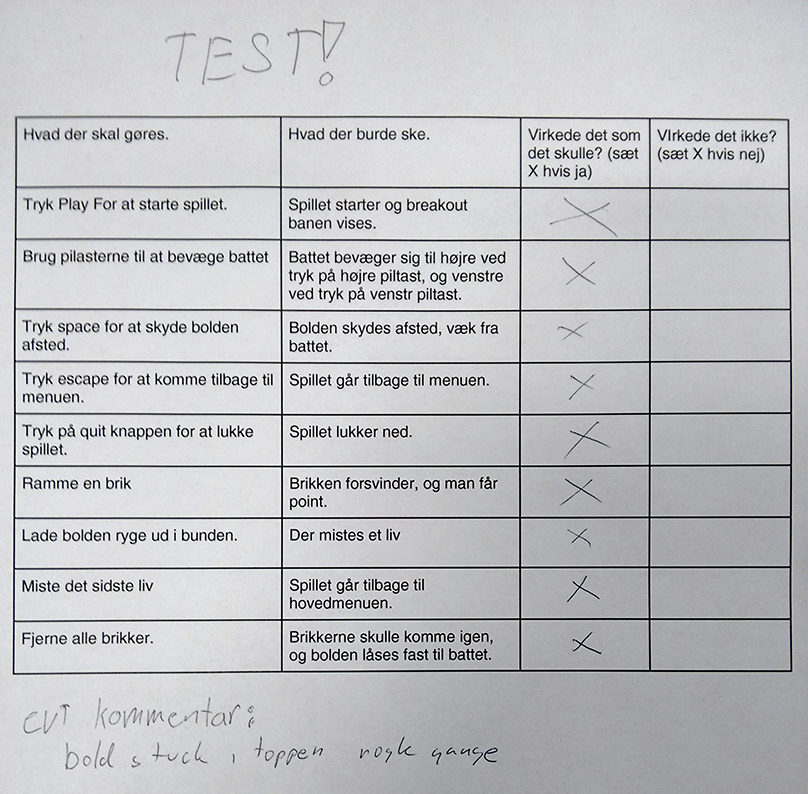
\includegraphics[width=0.98\linewidth]{pictures/testing/BlackboxTestArkBilag}
		\end{center}
\end{figure}